\documentclass{report}
\usepackage{tikz}

\begin{document}

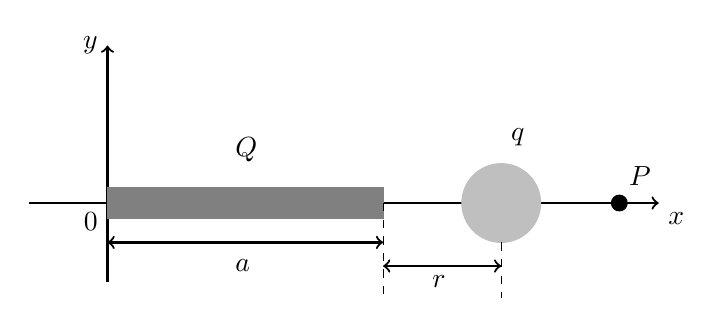
\begin{tikzpicture}[xscale=1, yscale=1]
%eixos
\draw [thick, ->]  (0,-1) -- (0,2);
\draw [thick, ->] (-1,0) -- (7,0);
\node [below right] at (7,0) {$x$};
\node [left] at (0,2) {$y$};
\node [below left] at (0,0) {$0$};

%barra
\draw [gray, fill=gray] (0,.2) rectangle (3.5,-0.2);
\node[above right] at (1.5,0.4) {$Q$};
%cota da barra
\draw [thick, <->]  (0,-0.5) -- (3.5,-0.5);
\node[below right] at (1.5,-0.6) {$a$};


%esfera
\draw[gray!50, fill=gray!50] (5,0) circle (.5);
\node[above right] at (5,0.6) {$q$};
%cota da esfera
\draw [thick, <->]  (3.5,-0.8) -- (5,-0.8);
\node[below right] at (4,-0.8) {$r$};

%ponto P
\draw[fill] (6.5,0) circle (.1);
\node[above right] at (6.5,0.1) {$P$};

%limite das cotas
\draw [dashed, -]  (3.5, 0) -- (3.5,-1.2);
\draw [dashed, -]  (5, -0.5) -- (5,-1.2);


\end{tikzpicture}


\end{document}